\scanpage{22}
\mspage{20}
% archive sheet number: 21
% hand: Grothendieck
% sheet_kind: text
% element: text | top, lines 1–3 | la représentation
la représentation \inserted{$u$} est \uline{quasi-unipotente} s'il existe un sous-groupe ouvert $U$ de $\pi$ tel que la représentation induite $u\mid U$ soit unipotente.

% element: text | upper-middle, lines 4–13 | 5.2 Supposons R infini
5.2. Supposons $R$ infini, et soit $G$ le groupe algébrique engendré par $u(\pi)$, \deleted{Alors} c.à.d. l'adhérence (avec structure induite réduite) de l'ens $u(G)$ dans le schéma en groupes des autom. de $E$. Comme l'ensemble des \deleted{\unsure{pts} de}\inserted{automorphismes} \deleted{\unsure{Aut}} unipotents \deleted{\unsure{constitue}}\inserted{est} une partie Zariski-fermée de l'ens $\operatorname{Aut}(E)$, il s'ensuit que $u$ est unipotent ssi $G$ est unipotent, (i.e. chacun de ses éléments \inserted{sur $\overline R$} est un automorphisme unipotent de $E_{\overline R}$).
% element: margin note | left margin, beside lines 11–14 | Noter que G/G^0
\margin{Noter que $G/G^\circ$ est un groupe \deleted{\unsure{et}} quotient isom. à $\pi/U$, où $U$ est l'image inverse de $G^\circ(R)$}

% element: text | middle-lower, lines 13–19 | 5.3 Si R est un corps
\deleted{\unsure{Dém.|De même}}\inserted{5.3.} Si $R$ est un corps topologique \inserted{séparé}, et $u$ est continue, alors dire que $u$ est quasi-unipotent revient à dire que $G^\circ$ est unipotent. C'est évidemment suffisant, car l'homomorphisme $\pi\longrightarrow(G/G^\circ)(R)$ \inserted{\unsure{ou} $G(R)/G^\circ(R)$} est continu \inserted{pour la top. discrète sur $G/G^\circ$}, donc l'image inverse de $G^\circ(R)$ est un sous-groupe ouvert \deleted{\unsure{de}} $U$ de $\pi$.
% element: drawing | lower left margin, beside lines 18–20 | tall loops, R and uncertain labels
% crop-candidate: scan 22
\figure{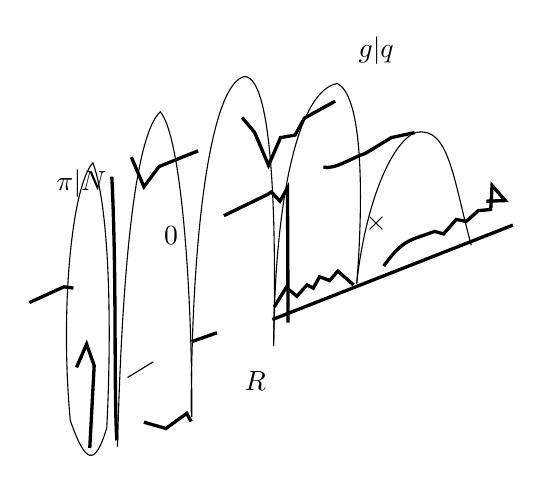
\begin{tikzpicture}[x=0.008cm,y=-0.008cm]
\draw[thin] (65,650)..controls(48,465)and(69,275)..(101,241)..controls(128,315)and(131,505)..(123,662)..controls(104,725)and(89,719)..(65,650);
\draw[thin] (140,692)..controls(147,419)and(167,197)..(208,160)..controls(243,200)and(259,464)..(258,645);
\draw[thin] (257,638)..controls(258,326)and(292,113)..(342,104)..controls(390,105)and(392,370)..(388,530);
\draw[thin] (388,532)..controls(390,288)and(429,126)..(489,115)..controls(537,138)and(527,350)..(520,433);
\draw[thin] (520,432)..controls(535,298)and(578,205)..(614,193)..controls(667,181)and(674,271)..(702,372);
\draw[very thick] (0,463)--(55,438)--(70,440);
\draw[very thick] (386,490)--(768,340);
\draw[very thick] (75,566)--(91,529)--(103,563)--(96,694);
\draw[very thick] (131,263)..controls(139,420)and(134,600)..(139,682);
\draw[very thick] (162,232)--(182,279)--(206,247)--(268,222);
\draw[very thick] (182,653)--(217,663)--(250,639)--(257,652);
\draw[very thick] (258,525)--(298,511);
\draw[very thick] (338,169)--(358,193)--(380,245)--(399,201)--(422,197)--(437,170)--(486,143);
\draw[very thick] (309,325)--(379,291)--(386,286);
\draw[very thick] (385,288)--(398,302)--(410,281)--(411,495);
\draw[very thick] (467,248)..controls(486,252)and(514,232)..(534,226)--(575,201)--(612,193);
\draw[very thick] (389,470)--(408,439)--(425,453)--(441,435)--(451,440)--(461,422)--(477,428)--(490,413)--(515,435);
\draw[very thick] (563,405)..controls(590,366)and(607,363)..(624,357)--(644,350)--(658,354)--(678,331)--(694,334)--(713,317)--(735,315);
\draw[very thick] (733,313)--(735,277)--(756,301)--(726,302);
\draw[thin] (156,582)--(197,557);
\node at(83,274){$\unsure{\pi|N}$};
\node at(359,588){$R$};
\node at(551,63){$\unsure{g|q}$};
\node at(225,356){$\unsure{0}$};
\node at(551,338){$\unsure{\times}$};
\end{tikzpicture}}
% element: text | bottom, lines 19–24 | Inversement
Inversement, si $U$ est un s-groupe ouvert de $\pi$ qui opère de façon unipotente, prenant $U$ assez petit on peut supposer que $U\subset u^{-1}(G^\circ(R))$. Alors $\overline{u(U)}$ est un sous-groupe algébrique \inserted{lisse $H$} de $G^\circ$, donc
